\title{Can multi-scale image pyramid processing concepts improve migration results?}
\author{Thomas Rapstine, Center for Wave Phenomena, Colorado School of Mines}

%\include{~/iTeam/Share/pcsmacros}

%\def\req{equation~\ref{eqn:#1}}
\def\req{equation~\ref}
\def\rfn#1{\ref{fig:#1}}


\maketitle
\inputdir{experiment}


%\begin{itemize}
%\item TODONE: Why is this project being done
%\item TODONE: What is the approach
%\item TODONE: What are the results
%\item TODONE: Give outline of paper
%\end{itemize}

\section{Introduction}

Analyzing images at multiple scales provides opportunities for image improvement, compression, and fusion with other images.  Seismic imaging using reverse time migration (RTM) results in valuable images of the subsurface.  This paper analyzes conventional RTM results at multiple image scales and compares conventional RTM results with alternative results using a multi-scale imaging condition.

I propose that an multi-scale analysis be performed on an RTM image resulting from the use of the CIC.  Furthermore, I propose that this multi-scale representation of an RTM image be used as a basis for developing a multi-scale imaging condition.  I hypothesize that leveraging multi-scale representations of source and receiver wavefield will provide a means to identify and suppress imaging artifacts such as cross-talk and back-scattering. 

In what follows, a basic theoretical background is given on both multi-scale image processing using image pyramids and on RTM.  A numerical experiment is then performed to gain understanding on the effects of scale on an RTM result and to evaluate a new imaging condition using image pyramids.

\section{Theory}

%\begin{itemize}
%\item TODONE: Theory on image pyramids
%\item TODONE: Mathematical representation of an image pyramid
%\end{itemize}

An image pyramid is a recursively derived multi-scale representation of a single image \cite[]{gonzalez2009digital}.  Just as a 2D signal can be decomposed into sines and cosines of varying frequencies using a Fourier transform, a 2D image can similarly be decomposed into various scales using an image pyramid.  Large scale components represent long wavelength components, while small scale components represent small wavelength components.  Each level of the pyramid is a lower resolution, larger scale, representation of the original image and contains less small scale, high frequency, signal.  To move up the pyramid, the image is first smoothed, to avoid aliasing, then subsampled.  Each level in the pyramid is constructed using the previous level, therefore the pyramid can be derived recursively.  As one moves up an image pyramid the image signal to noise improves as the larger scale features in the image are preserved while the small scale features are suppressed. 

To construct the pyramid, begin with the original image denoted as $\mathbf{G}_{0}$, where the subscript indicates the level in the pyramid.  Each level $j$ is constructed by operating upon the previous level $j-1$ for $j=1, \hdots , N_l$ where $N_l$ is the max level in the image pyramid.  The operation of moving up the pyramid to level $j$ is given in \req{eqn:pyrup},

\begin{equation} \label{eqn:pyrup}
\mathbf{G}_j=\mathbf{B}_{j-1}\mathbf{A}_{j-1}\mathbf{G}_{j-1}.
\end{equation}

Here, $\mathbf{A}_{j-1}$ is smoothing operator, and $\mathbf{B}_{j-1}$ is a subsampling operator on the image at level $j-1$.  The subsampling operator removes even rows and columns from the smoothed image.  Moving up the pyramid results in an image that is smaller with lower resolution but a higher signal-to-noise ratio resulting from smoothing.  The adjoint operator for moving up the pyramid is referred to as moving down the pyramid.  Moving down the image pyramid can be expressed using adjoint operators in \req{eqn:pyrdown},

\begin{equation} \label{eqn:pyrdown} 
\mathbf{G}_{j+1}=\mathbf{A}^T_{j}\mathbf{B}^T_{j}\mathbf{G}_{j}.
\end{equation}

The operator $\mathbf{B}^T_{j}$ injects zeros every other row and column; the operator $\mathbf{A}^T_{j}$ is the adjoint of the smoothing operator $\mathbf{A}_{j}$.  The notation $\mathbf{G}_{i,j}$ is used to indicate an image has been moved up the pyramid $i$-times and down $j$-times; implying that an image $\mathbf{G}_{3,3}$ has been moved down 3 times and then back up 3 times.  Information in an image is lost when moving down the pyramid.  The information lost at a particular level of the pyramid, referred hereafter as the residual at level $k$, is computed by moving the next level $k+1$ back down the image pyramid once:

\begin{equation} \label{eqn:residual}
\mathbf{L}_k = \mathbf{G}_k-\mathbf{G}_{k+1,1}.
\end{equation}

Here, the index $k$ ranges from 0 to $N_l-1$ since the image at the maximum level in the pyramid, $N_l$, is needed to compute the residual $\mathbf{L}_k$.  To reconstruct the image, the residuals $L_k$ and the highest level of the pyramid $\mathbf{G}_{N_l}$ are moved down the pyramid and summed

\begin{equation} \label{eqn:reconstruct}
\hat{\mathbf{G}}=\sum_{k=1}^{N_l-1}{\mathbf{L}_{k,k}} + \mathbf{G}_{N_l,N_l}.
\end{equation} 

It is advantageous to decompose an image into a pyramid to examine the image features at a variety of scales.  Luckily, the image pyramid is not much larger than the original image.  Each level of the pyramid is $\dfrac{1}{4}$ the size of the previous level.  An image of size $N$-by-$N$ results in an image pyramid size that can be computed using a geometric series 

\begin{equation}
N^2\left[\dfrac{1}{4}+\dfrac{1}{4^2}+\hdots+\dfrac{1}{4^P}+\right] = N^2\sum_{k=0}^{P} \left(\dfrac{1}{4}\right)^k \leq \dfrac{4}{3}N^2
\end{equation}

In my experience, reconstructing the image using \req{eqn:reconstruct} is mathematically sound but does not guarantee a perfect reconstruction.  This bothers me greatly, but I now accept the fact that building an image pyramid is a nonlinear operation.  Next, the concept of an image pyramid is applied to spatially decompose wavefields and images present in reverse time migration imaging.  A brief summary of the implementation specifics behind the RTM algorithm used in this paper follows.

In this paper, a variable density isotropic acoustic wave equation is implemented using finite differences.  It is implicitly assumed that density and velocity are slowly varying.  To perform RTM, first a source and receiver wavefield are constructed.  The source wavefield is constructed by injecting a source into a given density-velocity model and solving the previously mentioned wave equation over a predefined amount of time.  The receiver wavefield is constructed by reversing the data, injecting data as a source into a given density-velocity model, and subsequently reversing the time axis on the resulting wavefield \cite[]{baysal1983reverse}.  A conventional imaging condition (CIC), shown in \req{eqn:cic}, can then deployed to combine the source and receiver wavefields into an image of the subsurface denoted using $\mathbf{R}(\mathbf{x})$.  

\begin{equation} \label{eqn:cic}
\mathbf{R}(\mathbf{x})=\sum_t {\mathbf{W}_s(\mathbf{x},t)\mathbf{W}_r(\mathbf{x},t)}
\end{equation}



%\begin{itemize}
%\item TODONE: Give CIC 
%  \begin{itemize}
%    \item TODONE:  Note weaknesses of CIC 
%    \item TODONE:  Amplitudes are wack 
%    \item TODONE:  Crosstalk from Wr and Ws 
%    \item TODONE:  Mention EIC? 
%  \end{itemize}
%\end{itemize}

Conventionally, cross-correlation of source and receiver wavefield has been used as an imaging condition; this imaging condition is subsequently referred to as the conventional imaging condition (CIC).  The CIC is one option among many possible imaging conditions.  CIC is commonly used because of its simplicity and robustness, however the condition is not without pitfalls.  

First, a basic unit analysis on the CIC shows that it does not honestly preserve amplitudes.  When using the CIC, wavefield amplitudes are squared which results in exaggeration of high amplitude correlation in comparison to lower amplitude correlation.  A second notable pitfall of the CIC is a resulting imaging artifact so-called crosstalk.  Crosstalk is a result of undesirable correlation of source and receiver wavefields at locations not on a reflector at times before or after wavefields reach a reflector.  In my limited experience, generally speaking, crosstalk is a small scale localized high frequency artifact. A longer wavelength imaging artifact so-called back-scattering occurs when the source and receiver wavefield correlate at all depths along a path extending from the source to a reflector.

Given that cross-talk and backscattering artifacts occur at different scales, it is my hope that the artifacts can be suppressed by examining the wavefields at different scales to form an image.  There are three main options I see for utilizing the wavefields at different scales in an imaging condition: (1) weight based on scale alone, (2) weight based on scale and vary weight for either time or space, and lastly, (3) weight based on scale, time, and space.  In this paper, I choose to explore the simplest option (1) of scaling each level without considering varying time or space. 

An extension of the CIC to multiple image pyramid levels is introduced in \req{eqn:cic_level} to address large wavelength backscattering effects.  The resulting migrated image varies with scale denoted using $\mathbf{l}$, where $l_i$ is an entry of $\mathbf{l}$.  Each time step of the wavefields is treated as an image and is decomposed using the image pyramid theor discussed above.  I propose a new imaging condition in which decomposed source and receiver wavefields be weighted and summed to form a image as outlined in \req{eqn:cic_level_s}.  The weights of each scale are given by $\beta_i \in (0,1)$ $i=1,\hdots,N_l$ where all $\beta_i$ sum to one.  In the following section, this imaging condition is analyzed using a simple velocity and density model.

\begin{equation} \label{eqn:cic_level}
\hat{\mathbf{R}}_1(\mathbf{x},\mathbf{l})=\sum_t {\mathbf{W}_s(\mathbf{x},t,\mathbf{l})\mathbf{W}_r(\mathbf{x},t,\mathbf{l})}
\end{equation}


\begin{equation} \label{eqn:ws_hat}
\hat{\mathbf{W}}_s(\mathbf{x},t,l_i)=\beta_i\mathbf{W}_s(\mathbf{x},t,l_i)
\end{equation}

\begin{equation} \label{eqn:wr_hat}
\hat{\mathbf{W}}_r(\mathbf{x},t,l_i)=\beta_i\mathbf{W}_r(\mathbf{x},t,l_i)
\end{equation}

\begin{equation} \label{eqn:cic_level_s}
\begin{aligned}
\hat{\mathbf{R}}_2(\mathbf{x},l_i)
=&\sum_t {\hat{\mathbf{W}}_s(\mathbf{x},t,l_i)\hat{\mathbf{W}}_r(\mathbf{x},t,l_i)}\\
=&\beta_i^2\sum_t {\mathbf{W}_s(\mathbf{x},t,l_i)\mathbf{W}_r(\mathbf{x},t,l_i)}\\
=&\beta_i^2       \hat{\mathbf{R}}_1(\mathbf{x},l_i) 
\end{aligned}
\end{equation}

\section{Results}

First, I examine the effects of decomposing a migrated image using an image pyramid.  The resulting images are shown in figures \rfn{R_cic_l04_u}, \rfn{R_cic_l03_u}, and \rfn{R_cic_l01_u}.  This decomposition is performed after the migrated image is obtained using \req{eqn:cic}.  We see that detail is lost as the migrated image is represented at higher image pyramid levels.

Next, I examine migrated images resulting from a decomposition of each time step of the wavefield using a Gaussian pyramid according to \req{eqn:cic_level} for levels 0-4.  The results using decomposed wavefields are shown in figures \rfn{R_m_l04_u}, \rfn{R_m_l03_u}, and \rfn{R_m_l01_u}.  Again, we observe the loss of detail as we use higher pyramid levels for the wavefields for computing the migrated image.  However, the results obtained with decomposed wavefield are not identical to the migrated image results using a decomposed migrated image.  The images are not the same because of the nonlinearity of the image pyramid operation.  In general, one can not decompose and sum and expect the same results as summing and then decomposing an image.

In light of these results, I decided to try and weight different wavefield levels with a scalar value $\beta_i$, where subscript $i$ denotes the pyramid level index, before applying an imaging condition given in \req{eqn:cic_level_s}.  I chose to constrain the $\beta_i$ values to sum to one over all $i$.  I tried weighing lower levels in the pyramid more than higher levels in hopes of reducing long wavelength backscattering effects from contaminating the migrated image.  However, after a considerable amount effort I found that the resulting images were simply a weighted sum of the migrated results in \req{fig:decomp_cic}.  This is shown mathematically in \req{eqn:cic_level_s}.  Furthermore, the weighted results did not have attenuated backscattering effects given my naive and constraining criteria for the scaling parameter $\beta_i$.  This lead me to define a new, simpler, imaging condition in \req{eqn:cic_ws} that relies on a level-varying scalar value $\alpha_i$, where $\alpha_i$ is allowed to be any number in (-1,1).  The expanded bound in $\alpha_i$, compared to $\beta_i$, allows the truncation of levels.

\begin{equation} \label{eqn:cic_ws}
\hat{\mathbf{R}}_3(\mathbf{x})
=\sum_{\alpha_i} {\alpha_i \hat{{\mathbf{R}}}_1(\mathbf{x},l_i)}
\end{equation}

To demonstrate the imaging condition using scaled levels, the image results for truncating at various levels is shown in figures \rfn{Rh_m_k4}, \rfn{Rh_m_k3}, \rfn{Rh_m_k2}, and \rfn{Rh_m_k1}.  The results are unexpected and difficult to justify by intuition.  When truncating at level 4 a backscattering artifact still remains relatively strong; truncating at lower levels results in a slightly suppressed backscattering artifact.  

Another interesting feature of the resulting images is the variation in the definition of the flat reflector at 0.5 km and 0.75 km depth.  When truncating at levels 1 and 4, the flat events are well defined at a zero crossing in the image values; however truncating at levels 2 and 3 show more ambiguous reflection locations.  Additionally, the polarity of the event flips when comparing truncations at level 1 to level 4.  An undesirable effect of the truncated image results is the amplified migration swing extending from the reflector at 0.5 m depth.




% CIC then decompose R(x)
\multiplot{3}{R_cic_l04_u,R_cic_l03_u,R_cic_l01_u}{width=0.4\textwidth}{Compute image using CIC then decompose using image pyramid.  From top to bottom levels 4, 3, and 1 are shown.  Detail is lost as level increases as expected.}

% Decompose W_s and W_r and CIC on each level (Gaussian)
\multiplot{3}{R_m_l04_u,R_m_l03_u,R_m_l01_u}{width=0.4\textwidth}{Migrated images computed by first decomposing wavefields then using CIC, (see equation 7). From top to bottom pyramid levels 4, 3, and 1 are shown. Detail is still lost as level increases, but the results are different from figure \rfn{R_cic_l04_u} and company. }

% Results for truncating high levels
\multiplot{4}{Rh_m_k4,Rh_m_k3,Rh_m_k2,Rh_m_k1}{width=0.4\textwidth}{\label{fig:decomp_s_cic}Migrated image results for truncating levels according to \req{eqn:cic_ws} for truncation at levels 4, 3, 2, and 1, respectively from top to bottom.  Note polarity reversals at events and suppression of backscattering effects when truncationing at levels 3, 2, and 1. } 





\section{Conclusions}

The multi-scale imaging condition proposed in this paper has been implemented and the results are confusing at best.  The low frequency backscattering effects were not removed, but were attenuated when truncating specific levels of the image pyramid; the hypothesized benefits from using an image pyramid to attenuate backscattering effects have not been observed.  However, the results do show an oddly sharp event for flat reflectors in the migrated image.  Additional work is need to test if these sharp events remain when reflectors are dipping.  Future work could investigate using more sophisticated image pyramid decompositions using steerable filters or discrete wavelet transform.


\bibliographystyle{seg}
\bibliography{mybib}

% extra stuff 
%\inputdir{data}
%\plot{noise}{width=0.45\textwidth}{A plot of our signal.}
%\sideplot{spectra}{width=0.45\textwidth}{The amplitude spectrum of our signal.}
%
%\multiplot{2}{noise,spectra}{width=0.45\textwidth}{The signal (a), and the amplitude spectrum (b) plotted using multiplot (which is great for making large plots across columns).}


%\begin{figure}
%    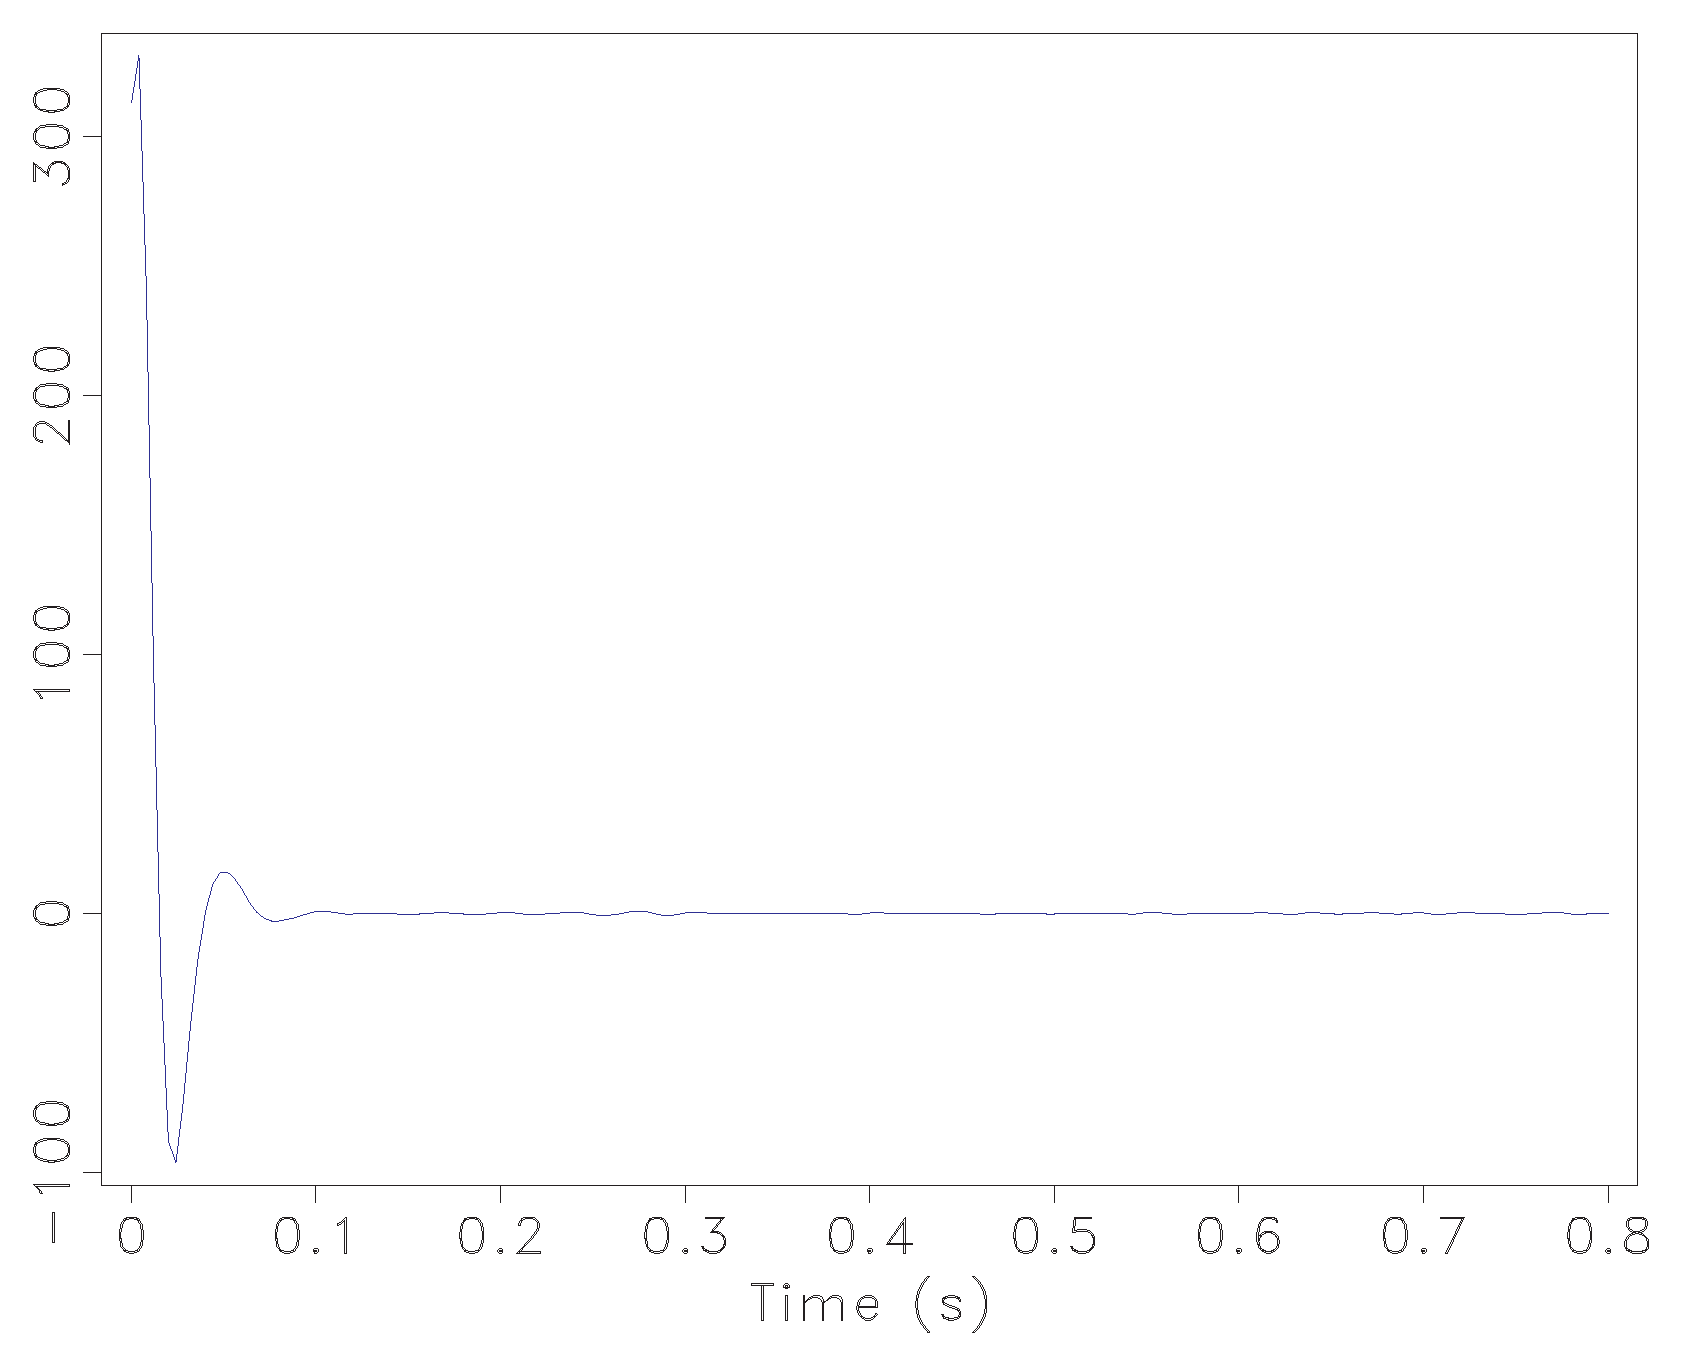
\includegraphics[width=0.45\textwidth]{data/Fig/noise} 
%    \caption{Earth}
%\label{Fig:core}
%\end{figure}
%\plot{Rh_m_ka}{width=0.4\textwidth}{}

% Decompose W_s and W_r and CIC on each level (Laplacian)
%\multiplot{3}{R_m_l04_u,R_m_l03_L_u,R_m_l02_L_u,R_m_l01_L_u}{width=0.4\textwidth}{decompose wavefields then CIC (Laplacian pyramid)}

% Truncated results truncate at 2, 3, 4, 5, 6
% TODO: (PLACEHOLDERS)
%\multiplot{3}{R_m_l04_u,R_m_l03_L_u,R_m_l02_L_u,R_m_l01_L_u}{width=0.4\textwidth}{Truncated at level two, three, and four respectively.}
%\multiplot{3}{R_m_l04_u,R_m_l03_L_u,R_m_l02_L_u,R_m_l01_L_u}{width=0.4\textwidth}{Truncated at level five, six, and seven.}


% CIC then decompose R(x)
%\multiplot{3}{R_cic_l04_u,R_cic_l03_u,R_cic_l02_u,R_cic_l01_u,R_m_l04_u,R_m_l03_u,R_m_l02_u,R_m_l01_u}{width=0.4\textwidth}{CIC then decompose}\label{fig:cic_decomp}
